\chapter{Angriffe}
\label{chap:attacks}
Um die Möglichkeiten potenzieller Angreifer und damit die möglichen Mitigation-Verfahren besser verstehen zu können werden nachfolgend die gängigsten Angriffe auf DNS beschrieben. Dabei wird spezieller Fokus auf für Clients relevante Gefahren gelegt. Angriffe die weder Vertraulichkeit, noch Integrität oder Verfügbarkeit des Clients gefährden werden bewusst nicht behandelt.

\section{DNS Sniffing}
\label{sec:attacks-dnssniffing}
Als Sniffing-Angriffe werden alle Arten von Angriffen bezeichnet die es ermöglichen Nachrichten zwischen mindestens 2 Parteien zu beobachten, mitzulesen und/oder mitzuhören\cite{CAPEC157}. In Hinblick auf DNS hat dies eine spezielle Bedeutung da es, aufgrund des fehlenden Schutz der Vertraulichkeit, ermöglicht, alle Informationen der Anfragen und Antworten einzusehen. Somit ist das Kommunikationsverhalten der Opfergeräte leicht nachzuvollziehen, was weiter Angriffe erheblich erleichtern kann. Das Aufzeichnen des DNS-Verkehrs lässt außerdem umfangreiche Schlussfolgerungen auf das Kommunikationsverhalten des Opfers zu. Darüber hinaus kann so auch die Transaktions-ID zusammen mit dem Ausgangsport erfahren werden, was die Voraussetzung für eine Spoofing-Attacke (siehe \ref{sec:attacks-dnsspoofing}) darstellt. 

\section{DNS Spoofing}
\label{sec:attacks-dnsspoofing}
\begin{wrapfigure}{r}{0.5\textwidth}
    \begin{center}
        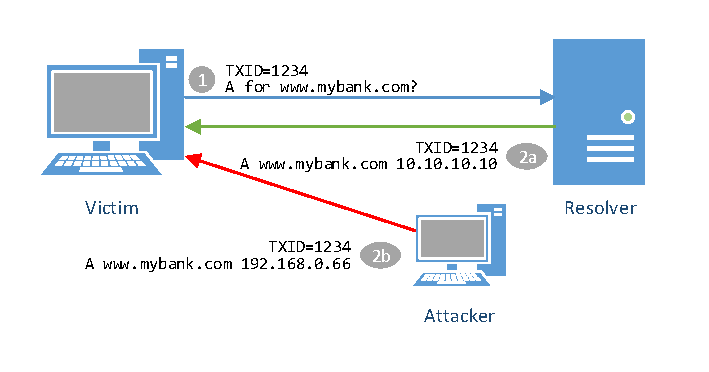
\includegraphics[width=0.48\textwidth,trim={8mm 8mm 8mm 8mm},clip]{DNS_Spoofing}
    \end{center}
    \caption{Darstellung einer klassischen DNS Spoofing Attacke.}
    \label{img:dnsspoofing}
\end{wrapfigure}

Spoofing Angriffe, auch \textit{Identity Spoofing} genannt, über die Aktion des ``zielgerichteten Glaubhaft machen einer gefälschten Identität'' definiert\cite{CAPEC151}. Es ist einem Angreifer dadurch möglich, dem Opfer falsche Informationen mitzuteilen, die als glaubwürdig und richtig behandelt werden. Im Fall von DNS spricht man von DNS Spoofing, was dieses simple Konzept auf einfache Art ausnützt.

Das DNS Netzwerkprotokoll verlässt sich beim Prüfen der Authentizität der Antworten nun einerseits auf das Transportprotokoll (meistens UDP) und eine 16-bit \ac{TXID} \cite{rfc1035}. Gelingt es einem Angreifer nun sowohl das ausgehende Port, als auch die \ac{TXID} in Erfahrung zu bringen, ist es einfach möglich eine gefälschte, glaubwürdige Antwort zu generieren (siehe Abb. \ref{img:dnsspoofing}). Kommt diese nun vor der echten Antwort beim Client an oder wird sogar vom Angreifer ganz abgefangen, kann dem Opfer jede beliebige Antwort glaubhaft gemacht werden.

\subsection{DNS Cache Poisoning}
DNS Spoofing ermöglicht es, den DNS-Cache eines Zielrechners aktiv zu manipulieren. Angriffe die Einträge in Caches von Opfern verändern, werden allgemein als \textit{Cache Poisoning}-Attacken bezeichnet\cite{CAPEC141}. \textit{DNS Cache Poisoning} bietet somit die Möglichkeit, gezielt gefälschte Einträge in die Caches von Servern einzubringen\cite{CAPEC142}. Dies ermöglicht es einem Angreifer Verbindungen zu bestimmten Zieldomänen umzuleiten oder stillzulegen. Wie in Abb. \ref{img:dnscachepoisoning} zu sehen ist, wird für eine erfolgreiche Attacke kein Zugriff auf das Netzwerk des Opfers benötigt. Nachdem der Client die Anfrage an seinen Resolver abgesetzt hat (1), wird die Adresse über den rekursiven Auflöseprozess ermittelt (2,3,4,5a). Ein Angreifer sendet nun Antworten mit der gefälschten Absenderadresse des autoritativen Nameservers an den Resolver (5b). Diese werden vom Resolver akzeptiert, sollte sie die richtige \ac{TXID} enthalten und zeitlich vor der echten Antwort ankommen. Aufgrund der geringen Entropie der \ac{TXID} (16-bit) ist das simple Erraten dieser ID zwar aufwendig aber durchführbar \cite{Son2010}. Wird die gefälschte Antwort vom Server nicht akzeptiert, erhält der Client die echte Antwort (6a). Gelingt jedoch das Einbringen der falschen Antwort, sendet der Resolver die gefälschte Adresse zurück (6b). Je nach erhaltener Antwort wählt der Host des Opfers den richtigen (7a) oder gefälschten (7b) Webserver als Ziel der Verbindung.    

\begin{figure}[htbp]
    \centering
    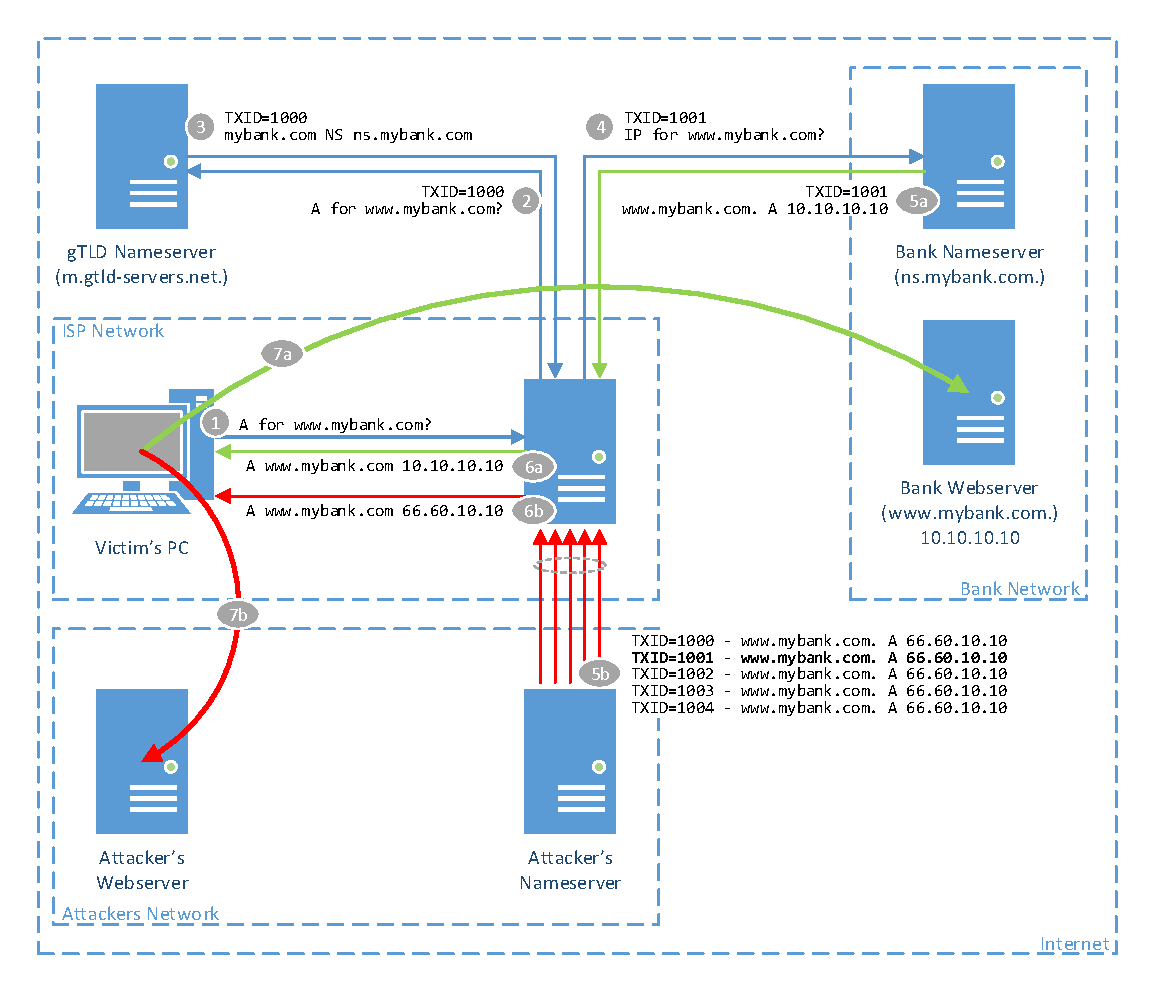
\includegraphics[width=0.8\textwidth]{DNS_CachePoisoning}
    \caption{Darstellung des Ablaufs einer DNS Cache-Poisoning Attacke}
    \label{img:dnscachepoisoning}
\end{figure}

\subsection{Kaminsky Angriff}
Eine viel gefährlichere Variante der Attacke ist 2008 vom amerikanischen Sicherheitsexperte Dan Kaminsky entwickelt worden\cite{Son2010}. In Abbildung \ref{img:dnskaminsky} wird gezeigt, wie es möglich ist, den Aufwand und die notwendige Zeit des Cache Poisoning massiv zu reduzieren. Dafür wird die Tatsache ausgenützt, dass die meisten Ziel-Resolver auch vom Angreifer erreichbar sind. Wird nun eine Anfrage zum Auflösen einer nicht existenten Unterdomäne der Zieldomäne an den Resolver gestellt (1) beginnt dieser mit der normalen Auflösung (2,3,4,5a). Da die Domäne nicht vorhanden ist, kann sie auch nicht in den Cache aufgenommen werden. Unterdessen sendet der Angreifer, wie im normalen Cache Poisoning auch, gefälschte Antworten an den Resolver (5b). Diese enthalten neben der Auskunft, dass die Domäne nicht existiert, einen zusätzlichen Eintrag der den Resolver über einen neuen Nameserver Eintrag informiert. Dieser gefälschter Eintrag enthält die Adresse eines Nameservers unter der Kontrolle des Angreifers. Ab diesem Zeitpunkt werden alle Anfragen an die Zieldomäne zum Nameserver des Angreifers weiterleiten. Dies stellt die effektive Übernahme der gesamten Domäne dar.

\begin{figure}[!hb]
    \centering
    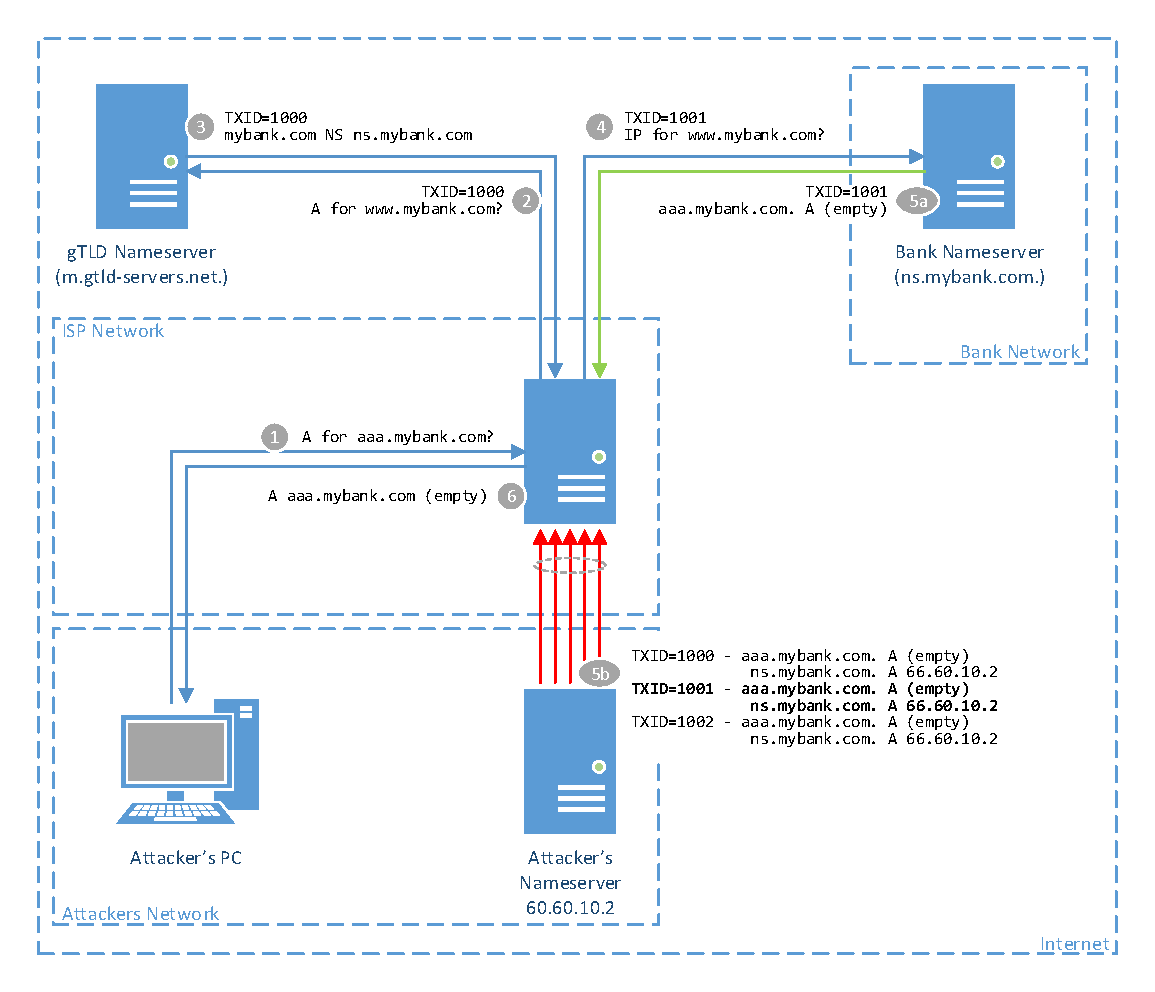
\includegraphics[width=0.8\textwidth]{DNS_Kaminsky}
    \caption{Schematische Darstellung des Ablaufs einer Kaminsky-Attacke}
    \label{img:dnskaminsky}
\end{figure}

Der Vorteil dieses Angriffs besteht in seiner beliebigen Wiederholbarkeit, da der eigentliche Eintrag nicht gecacht wird. Da der Auflöse-Prozess außerdem bewusst vom Angreifer initiiert wird, ist das korrekte Timing einfacher, die Attacke dadurch zuverlässiger.

\subsection{DNS Fragmentation Angriff}
Die Paketgröße der Vermittlungsschicht (OSI Layer 3) in Computernetzwerken ist limitiert, da die darunterliegende Sicherungsschicht (OSI Layer 2) nur Frames bis zu einer bestimmten Größe übertragen kann. Der limitierende Wert wird \ac{MTU} genannt und liegt in Ethernet-Netzwerken üblicherweise bei 1500 Bytes. Aufgrund dieser Beschränkung müssen Datagramme höherer Schichten, welche die MTU überschreiten, auf mehrere Unterpakete aufgeteilt werden. Dieser Vorgang wird als \textit{Fragmentierung} bezeichnet und kann für eine spezielle DNS Spoofing Attacke ausgenützt werden.

Bei DNS Spoofing muss der Angreifer die DNS \ac{TXID} (16-bit) erraten oder kennen. Nutzt man nun den Umstand der Fragmentierung, kann diese Unbekannte gegen einen andere, die IP-Fragment-Identification (IP-ID; 16-bit) getauscht werden. Der Vorteil dabei besteht in der besseren Vorhersagbarkeit dieser IP-ID, da sie ausschließlich vom antwortenden Server gewählt wird. Dies macht es für einen Angreifer einfach den Auswahlalgorithmus des Ziels genau zu studieren. Paart man diese Schwachstelle nun mit den Techniken der anderen Angriffe, erhält man eine überaus effektive Möglichkeit DNS Caches zu manipulieren \cite{Herzberg2013}.

\section{Man-In-The-Middle Angriff}
\label{sec:attack-mitm}
Wie viele ältere Protokolle ist auch DNS von einer starken Anfälligkeit gegen sogenannte \ac{MITM} Attacken betroffen. Diese Art des Angriffs zeichnet sich durch den Umstand aus, dass sich der Angreifer unbemerkt zwischen zwei Kommunikationsteilnehmer Positionieren kann \cite{CAPEC94}. Aufgrund seiner vermittelnden Position ist er in der Lage die Kommunikation zwischen den Teilnehmern komplett zu kontrollieren. Sollte er sich zwischen Endgerät und Recursive Resolver befinden, kann jede DNS-Interaktion nach Belieben manipuliert werden. Solle es dem Angreifer gelingen, sich vor einem autoritativem DNS-Server zu stellen, können alle Anfragen und Antworten an die von diesem Server bereitgestellten Domänen, manipuliert werden. 

Da dieser Angriff derartig mächtig ist, bieten sich jedoch oft effektivere Wege um die Kontrolle über die Ziele auszuweiten. Die genauen Angriffswege und Möglichkeiten der Ausnutzung werden von Conti, Dragoni und Lesyk \cite{Conti2016} ausführlich beschrieben und würden den Rahmen dieser Arbeit sprengen.

\section{Denial-Of-Service Angriff}
\label{sec:attacks-dos}
\ac{DoS} Attacken  zielen darauf ab die Nutzung bestimmter Dienstleistungen, Funktionen oder Geräte zu verhindern \cite{BSIG040}. Durch einen solchen Angriff auf den verwendeten Resolver oder relevante, autoritative DNS-Servern können kritischen Unternehmensdienste kurzfristig außer Betrieb genommen werden. In den meisten Fällen wird für die Angriffe auf DNS die DNS-Infrastruktur selbst herangezogen. Ist es bei klassischen \ac{DoS} Attacken noch einfach die sendenden Hosts über Firewalls oder Routing stillzulegen, so kann das Blockieren von DNS-Servern unvorhergesehene Auswirkungen auf die Funktionsweise des gesamten DNS haben\cite{Kambourakis2008}. 

\subsection{DoS-Amplification Angriff}
\label{sec:attack-dosamp}
\begin{wrapfigure}{r}{0.35\textwidth}
    \begin{center}
        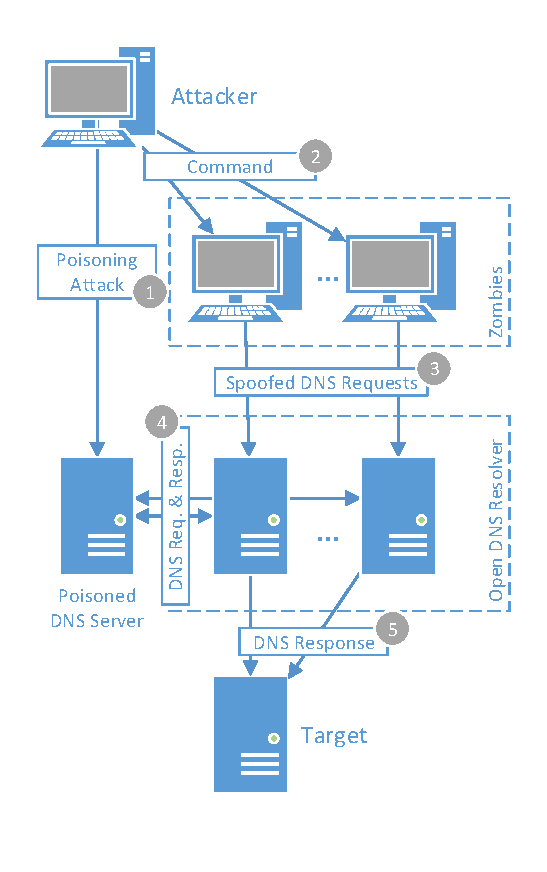
\includegraphics[width=0.33\textwidth,trim={5mm 10mm 5mm 10mm},clip]{DNS_DoS}
    \end{center}
    \caption{Darstellung eines DoS Angriffs mit DNS-Amplification.}
    \label{img:dnsdos}
\end{wrapfigure}

Die Nutzbarkeit von DNS als Verstärker (Amplifier) von \ac{DoS} Attacken ist schon länger bekannt und wurde auch schon früher als Problem erkannt \cite{ICANN2006}. Das Problem liegt hier an dem eingesetztem Transportprotokoll UDP zusammen mit dem Umstand, dass DNS keinerlei Authentifizierung des Clients verlangt. Sendet ein Angreifer nun ein Paket mit gefälschter Absenderadresse an einen DNS-Resolver so wird dieser eine entsprechende Antwort an den vermeintlichen Absender schicken. Wird nun eine große Anzahl an solchen Anfragen an mehrere Resolver gestellt, kann dies schnell zu einer teilweisen oder vollständigen Sättigung der Bandbreite des gewählten Ziels führen. Die Kommunikationsfähigkeit des Opfers kann somit erheblich beeinträchtigt werden, was zu einem \ac{DoS} führen kann. 

Verschärfend kommt hinzu, dass der übliche maximale Verstärkungsfaktor von 12,8 mittels \ac{DNSSEC} (siehe \ref{sec:tec-dnssec}) auf durchschnittlich 47,2 erhöht werden kann. Dies ist auf die mit \ac{DNSSEC} eingeführte Erweiterung EDNS0 zurückzuführen, die es ermöglicht größere Antwortpakete anzufragen. Es konnte gezeigt werden, dass beim Nutzen aller Möglichkeiten einen maximalen Verstärkungsfaktor von 102,4 möglich ist\cite{VanRijswijk-Deij2014}. Mit dieser Verstärkung wäre ein Angreifer mit 100Mbit/s Bandbreite dazu in der Lage ca. 10Gbit/s Traffic zu generieren.

\paragraph{}
Effektive Angriffe machen sich die beschriebene hohen Verstärkungsrate und geringen Transparenz des Systems zu Nutze \cite{Kambourakis2008}. Ein Angriff kann nun wie folgt ablaufen (siehe Abb. \ref{img:dnsdos}):
\begin{enumerate}[topsep=0pt,itemsep=-1ex,partopsep=1ex,parsep=1ex]
    \item Ein Angreifer bringt über Cache Poisoning einen speziellen RR (Amplifying Record) in einen Zielserver ein, der eine maximal große Antwort erzeigt.
    \item Einem zuvor gebildeter Bot-Netz wird nun das Kommando zum Anfragen dieses speziellen RR erteilt. 
    \item Es wird dabei ein DNS-Request mit gefälschter Absende-Adresse des Ziel an verschiedene offene Resolver gesendet.
    \item Die Resolver fragen nun den manipulierten Eintrag am und erhalten eine große Antwort.
    \item Da die Absende-Adresse gefälscht wurde, werden die Antworten an das Opfer gesendet und nehmen aufgrund ihrer Größe und Anzahl einen großen Anteil der Bandbreite ein. 
\end{enumerate}
Werden nun stetig neue Anfragen gestellt und eine ausreichend hohe Anzahl an Zombie-Rechnern bzw. Resolvern verwendet, kann die gesamte Bandbreite des Opfers saturiert werden. Dies stellt den als \ac{DoS} bezeichneten Zustand dar.

\section{DNS Rebinding}
\label{sec:attack-dnsrebind}
Eine weniger bekannte Art die Schwachstellen von DNS auszunutzen ist das sogenannte \textit{DNS Rebinding}. Ziel des Angriffs besteht im Überwinden der als \textit{Access Within Same Origin Policy} genannte Sicherheits-Technik moderner Browser. Diese verbietet es Scripts einer Webseite auf Inhalte zuzugreifen die nicht unter dem selben Hostnamen erreichbar sind. Es können zwar Ausnahmen definiert werden, da dies jedoch am Ziel passieren muss, besteht dadurch keine Gefahr. Die Schwachstelle besteht nun im Fakt, dass DNS-Einträge mit sehr geringer TTL gesetzt werden können. Es wird dadurch möglich die Adresse eines Namens während der Ausführung eines Scripts zu verändern\cite{Jackson2009}. Das ermöglicht den folgenden Ablauf.

\begin{enumerate}
    \item Das Opfer wird vom Angreifer auf eine von ihm kontrolliere Website gelockt. Der Nameserver des Angreifers vergibt für den DNS-Eintrag des Webservers eine sehr geringe TTL.
    \item Der Browser des Opfers führt die auf der Webseite eingebunden Scripts aus. Gleichzeitig läuft die TTL des gecachten Eintrags aus, was den Resolver zu einer erneuten Auflösung bewegt. Bei dieser wird nun vom Nameserver des Angreifers die Adresse eines Ziels zurück geliefert.
    \item Nach diesem \textit{Rebinding} des Hostnamen kann das laufende Script über den eigenen Namen auf die Ressourcen der Adresse des Ziels zugreifen. Dies erlaubt dem Script z.B. Zugriffe auf netzinterne Ressourcen wie Administrationsoberflächen oder ermöglicht das Scannen des LANs. Außerdem wird damit der Browser des Opfers für andere Angriffe, wie \ac{DoS} Attacken, nutzbar.   
\end{enumerate}

Auch wenn es viele Gegenmaßnahmen in aktuellen Browsern gibt und einige der anfälligen Komponenten (Java Applets, Flash, etc.) an Verbreitung verlieren, besteht besonders durch die zunehmende Verbreitung von IoT-Geräten eine akute Bedrohung durch diesen Angriffsweg\cite{Dorsey2018}. 

\section{BitSquatting}
Eine weitere, ausgefallene Angriffsmöglichkeit bietet das sogenannte \textit{BitSquatting}. Bei diesem Angriff werden zufällige Fehler im Hauptspeicher von Geräten ohne fehlererkennende Speichermodule ausgenützt. Es konnte gezeigt werden, dass es durch solche Fehler zum stellen fehlerhafter Anfragen an potenziell existente Domänen kommen kann\cite{Dinaburg2011}. Dieser Effekt kann nun bewusst ausgenutzt werden, indem eine große Anzahl an Domänen registriert werden, deren Name sich nur um ein Bit von viel besuchten Domänen unterscheidet (siehe Listing \ref{lst:bitquatting}). 
Da es in diesem Fall zu stellen falschen Anfragen kommt, gibt es auch keine Möglichkeit sich auf Protokoll- bzw. System-Ebene zu schützen. Die einzige effektive Lösung stellt der Einsatz von \textit{Error-correcting code memory} Hardware dar.  
\begin{lstlisting}[caption={Drei mögliche BitSquatting-Domänen für die Zieldomäne \texttt{amazon.com}}, label={lst:bitquatting}]
amazon.com = 61   6d   61 7a   6f   6e 2e 63 6f 6d
           ... 01101101 ... 01101111 ... 
aeazon.com = 61   65   61 7a   6f   6e 2e 63 6f 6d  
           ... 01100101 ...
                   ^
a-azon.com = 61   e2   61 7a   6f   6e 2e 63 6f 6d 
           ... 00101101 ...
                ^
amazgn.com = 61   6d   61 7a   67   6e 2e 63 6f 6d
                        ... 01100111 ...
                                ^
\end{lstlisting}

\section{Übersicht}
Gruppiert man nun die oben gezeigten Angriffe nach den in Kapitel \ref{chap:threads} beschriebenen Schwächen erhält man die in Abbildung \ref{img:attacks-summary} dargestellte Zuordnung. DNS Rebinding und BitSquatting wurden dabei als spezielle Attacke gesondert betrachtet.

\begin{figure}[!hb]
    \centering
    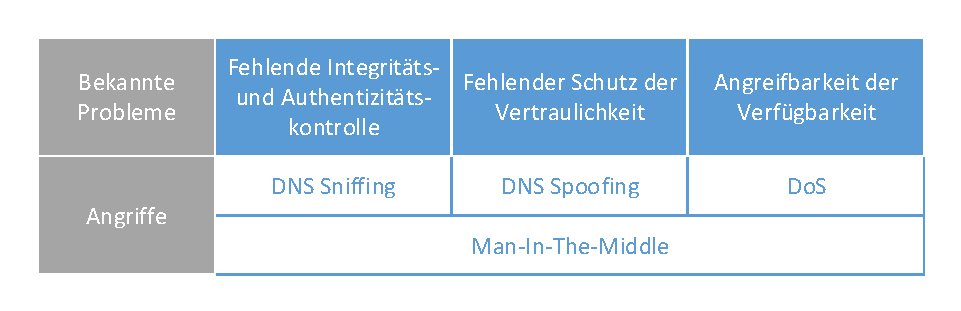
\includegraphics[width=\textwidth]{Overview_Attacks}
    \caption{Übersicht des Bezugs zwischen den vorgestellten Sicherheits-Problemen und den Attacken die diese ausnutzen.}
    \label{img:attacks-summary}
\end{figure}

